\documentclass[usenames,dvipsnames]{beamer}
%
% Choose how your presentation looks.
%
\usepackage[T1]{fontenc}
\usepackage[utf8]{inputenc}
\usepackage{lmodern}  
\usepackage{tikz}%boxy s vysvetlivkami 
\usetikzlibrary{calc}
\usepackage{amsmath}
\usepackage{bm}
\usepackage{color}
%
% For more themes, color themes and font themes, see:
% http://deic.uab.es/~iblanes/beamer_gallery/index_by_theme.html
%
\mode<presentation>
{
  \usetheme{Darmstadt}      % or try Darmstadt, Madrid, Warsaw, ...
  \usecolortheme{default} % or try albatross, beaver, crane, ...
  \usefonttheme{serif}  % or try default, serif, structurebold, ...
  \setbeamertemplate{navigation symbols}{}
  \setbeamertemplate{caption}[numbered]
  \setbeamertemplate{headline}{}
} 
%
%
\newcommand{\mytikzmark}[2]{%
  \tikz[remember picture,inner sep=0pt,outer sep=0pt,baseline,anchor=base] 
    \node (#1) {\ensuremath{#2}};}
%
%
\title[Week9]{Week 9: Simultaneous Equation Models and Miscellaneous Topics}
\author{Advanced Econometrics 4EK608}
\institute{Vysoká škola ekonomická v Praze}
\date{}

\begin{document}

\setlength{\abovedisplayskip}{1pt}
\setlength{\belowdisplayskip}{1pt} 
\setlength{\abovedisplayshortskip}{1pt}
\setlength{\belowdisplayshortskip}{1pt}

\begin{frame}
  \titlepage
\end{frame}
%---------------------------------------------
% Uncomment these lines for an automatically generated outline.
\begin{frame}{Outline}
  \tableofcontents
\end{frame}

%---------------------------------------------
\section{Introduction}
\begin{frame}{Introduction}
\underline{\textbf{Simultaneity is another important form of endogeneity}}\\
\bigskip
Simultaneity occurs if at least two variables are jointly determined. A typical case is when observed outcomes are the result of separate behavioral mechanisms that are coordinated in an equilibrium. 
\medskip
\\Prototypical case: a system of demand and supply equations:
\begin{itemize}
\item $D(p) $ how high \textit{would} demand be if the price was set to $p$?
\item $S(p) $ how high \textit{would} supply be if the price was set to $p$?
\vspace{0.2cm}
\item Both mechanisms have a ceteris paribus interpretation.
\item Observed quantity and price will be determined in equilibrium, where $D(p)=S(p)$.
\end{itemize}
\medskip
Simultaneous equations systems can be estimated by 2SLS/IVR\\
\dots ~Identification conditions apply.
\end{frame}
%---------------------------------------------
\begin{frame}{Examples}
\textcolor{Blue}{Example 1:} Labor supply and demand in agriculture \\
\bigskip
\qquad $h_s  = \alpha_1 w + \beta_1 z_1 + u_1$ \\
\qquad $h_d  = \alpha_2 w + \beta_2 z_2 + u_2$ \\
\begin{itemize}
\item Endogenous variables, exogenous variables, \\observed and unobserved supply shifter, \\observed and unobserved demand shifter\\
\medskip
\item We have $n$ regions, market sets equilibrium price and quantity in each. We observe the equilibrium values only \\
\vspace{0.3cm}
$h_{is} = h_{id} \Rightarrow (h_i, w_i)$
\end{itemize}
\end{frame}
%---------------------------------------------
\begin{frame}{Examples}
\textcolor{Blue}{Example 1:} Labor supply and demand in agriculture contnd.\\
\bigskip
\begin{itemize}
\item [] $h_i  = \alpha_1 w_i + \beta_1 z_{i1} + u_{i1}$
\item [] $h_i  = \alpha_2 w_i + \beta_2 z_{i2} + u_{i2}$ \\
\medskip
\item If we have the same exogenous variables in each equation, we cannot identify (distinguish) equations. \\
\medskip
\item We assume independence between errors in structural equations \& exogenous regressors. 
\end{itemize}
\end{frame}
%---------------------------------------------
\section{Simultaneity Bias}
\begin{frame}{Examples}
\textcolor{Blue}{Example 1:} Labor supply and demand in agriculture contnd.\\
\bigskip
If we estimate the structural equation with OLS method, estimators will be biased – so called ``simultaneity bias''. \\
\medskip
\quad \ $y_1  = \alpha_1 y_2 + \beta_1 z_1 + u_1 $ \\
\medskip
\quad \ $y_2  = \alpha_2 y_1 + \beta_2 z_2 + u_2 $ \\
\bigskip
$y_2$ is dependent on $u_1$ \\
(substitute RHS of the $1^{st}$ equation for $y_1$ in the $2^{nd}$ eq.)\\
\medskip
$\Rightarrow y_2  = \bigg[ \frac{\alpha_2 \beta_1}{1-\alpha_2 \alpha_1} \bigg] z_1 + \bigg[ \frac{\beta_2}{1 - \alpha_2 \alpha_1} \bigg] z_2 + \bigg[\frac{\alpha_2 u_1 + u_2}{1-\alpha_2 \alpha_1} \bigg] $ \\
\end{frame}
%---------------------------------------------
\begin{frame}{Structural and reduced form equations, 2SLS method}
\textbf{Structural equations} (example)\\
\medskip
\quad \ $y_1  = \beta_{10} + \beta_{11} y_2 + \beta_{12} z_1 + u_1 $ \\
\medskip
\quad \ $y_2  = \beta_{20}+\beta_{21} y_1 + \beta_{22} z_2 + u_2 $ \\
\bigskip
\textbf{Reduced form equations}\\
\medskip
\quad $y_1 = \pi_{10} + \pi_{11} z_1 + \pi_{12} z_2 + \varepsilon_1 \qquad 
\Rightarrow  \qquad \hat{y}_1~~$by OLS\\
\medskip
\quad $y_2 = \pi_{20} + \pi_{21} z_1 + \pi_{22} z_2 + \varepsilon_2 \qquad 
\Rightarrow  \qquad \hat{y}_2~~$by OLS\\
\bigskip
\textbf{2SLS} (a special case of IVR)\\
\begin{itemize}
\item $1^{st}$ stage: Estimate reduced forms, get $\hat{y}_1$ and $\hat{y}_2$.
\item $2^{nd}$ stage: Replace endogenous regressors in structural equations by fitted values from $1^{st}$ stage, estimate by OLS.\\
\medskip
\item \dots ~Identification of structural equations, \\
\dots ~Statistical inference in structural equations ($2^{nd}$ stage).
\end{itemize}
\end{frame}
%---------------------------------------------
\begin{frame}{Examples}
\textcolor{Blue}{Example 2: (Structural equations)} \\Estimation of murder rates\\
\medskip
\qquad $\textit{murdpc} = \beta_{10} + \alpha_1 \textit{polpc} +  \beta_{11} \textit{incpc} + u_1$ \\
\qquad \hspace{0.25cm} $\textit{polpc} = \beta_{20} + \alpha_2 \textit{murdpc} + \bm{\beta} (\textit{other factors}) + u_2$ \\
\medskip
\begin{itemize}
\item $1^{st}$ equation describes the behaviour of murderers, \\$2^{nd}$ one the behaviour of municipalities. \\Each one has its ceteris paribus interpretation.\\
\medskip
\item For the municipality policy, the $1^{st}$ equation is interesting: what is the impact of exogenous increase of police force on the murder rate? 
\item However, the number of police officers  is not exogenous (simultaneity problem). 
\end{itemize}
\end{frame}
%---------------------------------------------
\section{Identification problem}
\begin{frame}{Identification problem}
\textcolor{Blue}{Example 3: (Identification)}\\
Identification problem in a SEM\\ 
\vspace{0.5cm}
\begin{itemize}
\item Example: Supply and demand for milk
\end{itemize}
\qquad Supply of milk: \qquad $q = \alpha_1 p + \beta_1 z_1 + u_1$ \\
\qquad Demand for milk: \quad $q = \alpha_2 p + u_2$ \\
\medskip
\begin{itemize}
\item Supply of milk cannot be consistently estimated because we do not have (at least) one exogenous variable  ``available'' to be used as instrument for $p$ in the supply equation.\\
\medskip
\item Demand for milk can be consistently estimated because we can use exogenous variable $z_1$  as instrument for $p$ in the demand equation.
\end{itemize}
\end{frame}
%---------------------------------------------
\begin{frame}{Identification problem}
\begin{itemize}
\item Ilustration 
\end{itemize}
\medskip
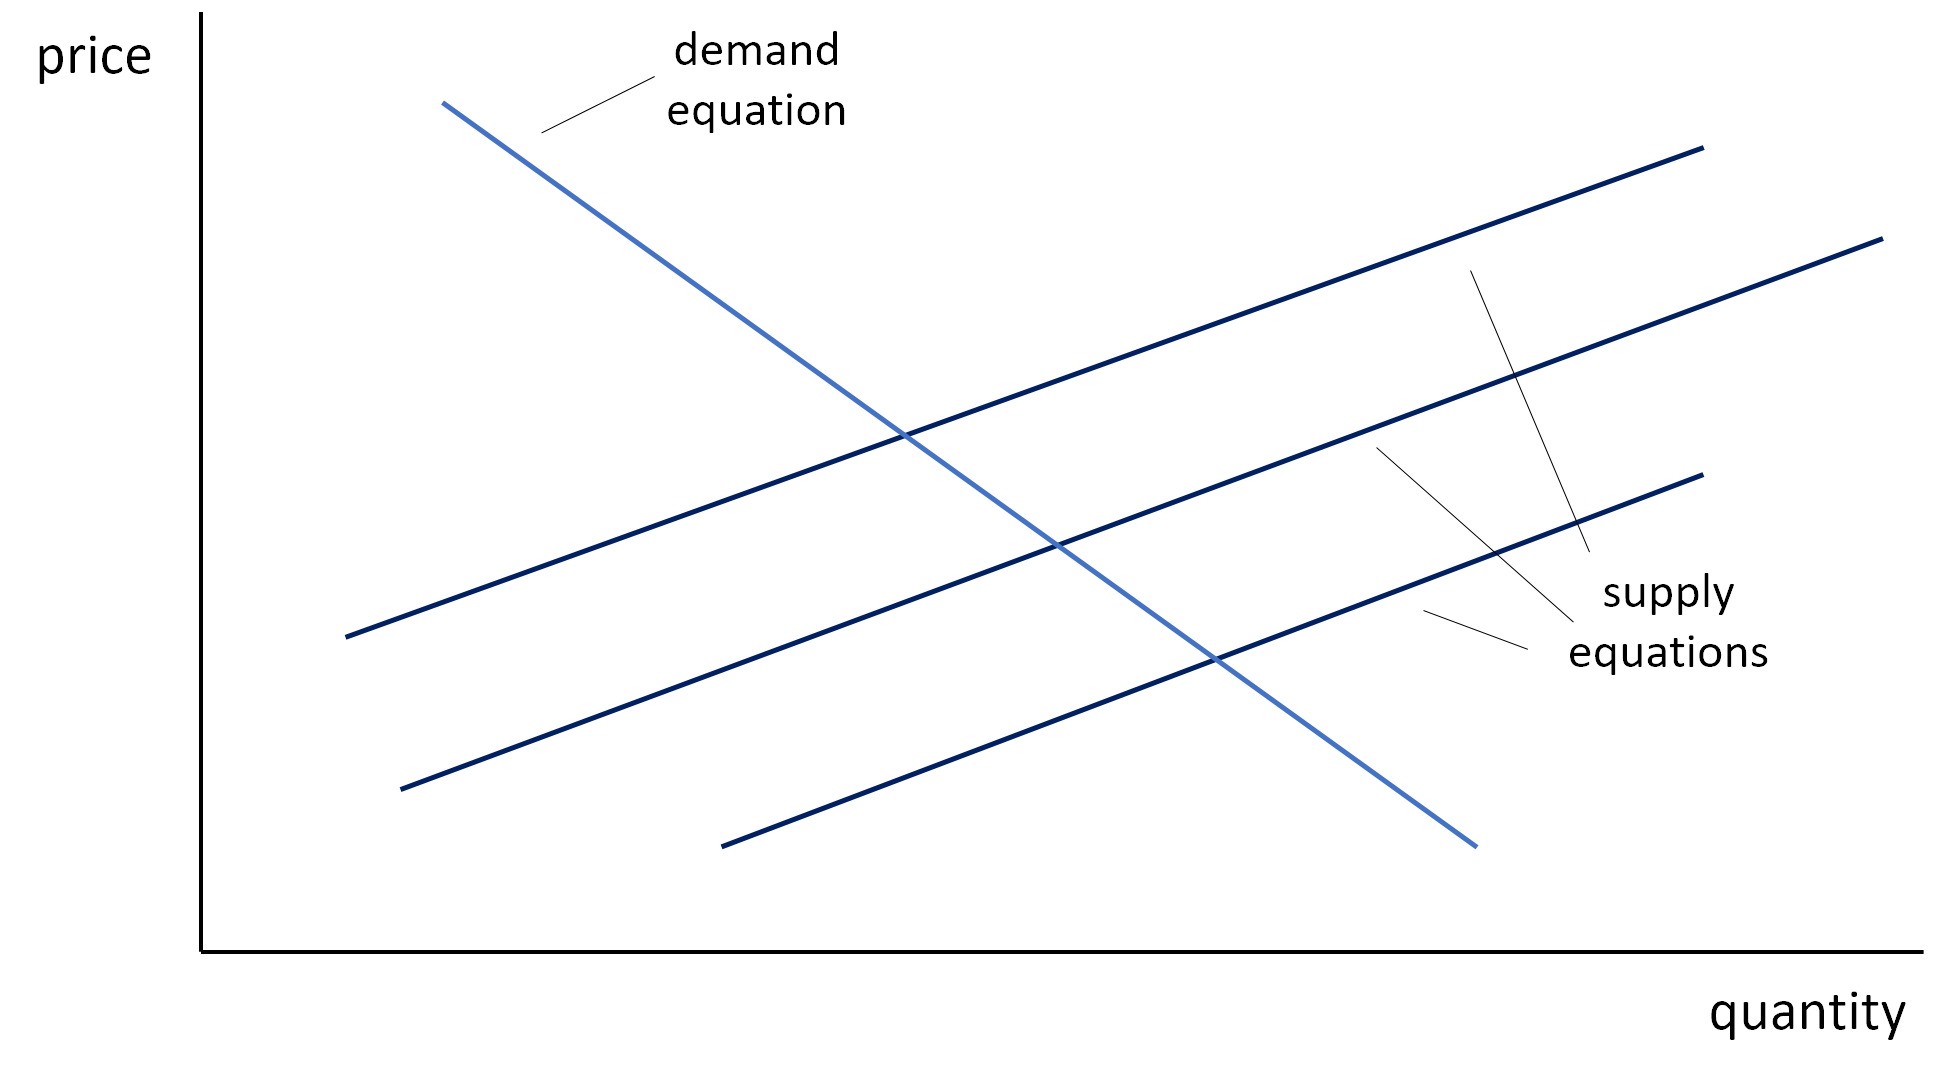
\includegraphics[width=\textwidth]{./img/W9_Obrazek_1}
\end{frame}
%---------------------------------------------
\section{Identification conditions}
\begin{frame}{Identification conditions}
Identification conditions for a sample 2-equation SEM \\(individual $i$ subscripts omitted)\\
\vspace{0.3cm}
\qquad $y_1 = \beta_{10} + \alpha_1 y_2 + \beta_{11} z_{11} + \beta_{12} z_{12} + \dots + \beta_{1k} z_{1k} + u_1$\\
\qquad $y_2 = \beta_{20} + \alpha_2 y_1 + \beta_{21} z_{21} + \beta_{22} z_{22} + \dots + \beta_{2k} z_{2k} + u_2$\\ 
\medskip
\begin{itemize}
\item  Order condition (necessary): $1^{st}$ equation is identified \\if at least one exogenous variable $z$ is excluded from $1^{st}$ equation (yet in the SEM).
\item Rank condition (necessary and sufficient): $1^{st}$ equation is identified if and only if the second equation includes at least one exogenous variable excluded from the first equation with a nonzero coefficient, so that it actually appears in the reduced form. 
\item For the second equation, the conditions are analogous.
\item Some estimation approaches allow for identification through IVs not explicitly included in the SEM.
\end{itemize}
\end{frame}
%---------------------------------------------
\begin{frame}{Examples}
\textcolor{Blue}{Example 4: (Identification)}\\ Labor supply of married working women\\
\bigskip
Supply (workers): 
\vspace{0.1cm}
\begin{flalign*}
\textit{hours} = \alpha_1 \log(\textit{wage}) & + \beta_{10} + \beta_{11} \textit{educ} + \beta_{12} \textit{age} + \beta_{13} \textit{kidslt}6 && \\
 & + \beta_{14} \textit{nwifeinc} + u_1 &&
\end{flalign*} \\
\medskip
Demand (enterprises):
\smallskip
\begin{flalign*}
\log(\textit{wage}) = & \alpha_2 \textit{hours} + \beta_{20} +\beta_{21} \textit{educ} + \beta_{22} \textit{exper} + \beta_{23} \textit{exper}^2 + u_2 && \\
\end{flalign*}
Order condition is fulfilled in both equations.
\end{frame}
%---------------------------------------------
\begin{frame}{Examples}
\textcolor{Blue}{Example 4: (Identification)}\\ Labor supply of married working women contnd.\\
\bigskip
\begin{itemize}
\item To evaluate the rank condition for supply equation, we estimate the reduced form for $\log(\textit{wage})$ and test if we can reject the null hypothesis that coefficients for both coefficients for $exper$ and $\textit{exper}^2$ are zero. \\If $H_0$ is rejected, the rank condition is fulfilled.\\
\medskip
\item We would do the evaluation of the rank condition for the demand equation analogically.
\end{itemize}
\end{frame}
%---------------------------------------------
\begin{frame}{Estimation}
\begin{itemize}
\item We can consistently estimate identified equations with the 2SLS method. \vspace{0.2cm}
\item In the $1^{st}$ stage, we regress each endogenous variable on all exogenous variables (``reduced forms'').
\vspace{0.2cm}
\item In the $2^{nd}$ stage we put into the structural equations instead of endogenous variables their predictions from the $1^{st}$ stage and estimate with the OLS method. 
\vspace{0.2cm}
\item The reduced form can be always estimated (by OLS).
\vspace{0.2cm}
\item In the $2^{nd}$ stage, we cannot estimate unidentified structural equations. 
\vspace{0.2cm}
\item With some additional assumptions, we can use a more efficient estimation method than 2SLS: 3SLS.
\end{itemize}
\end{frame}
%---------------------------------------------
\section{Systems with more than two equations}
\begin{frame}{Systems with more than two equations}
\textcolor{Blue}{Example 5:} Keynesian macroeconomic model
\vspace{0.2cm}
\begin{align*}
C_t & = \beta_0 + \beta_1(Y_t - T_t) + \beta_2 r_t + u_{t1} \\
I_t & = \gamma_0 + \gamma_1 r_t + u_{t2} \\
Y_t & \equiv C_t + I_t + G_t \\
\end{align*}
\vspace{-0.2cm}
\noindent Endogenous: $C_t, I_t, Y_t$ \hfill Exogenous: $T_t, G_t, r_t $ \\ 
\medskip
\begin{itemize}
\item Order condition for identification is the same as for two equations systems, rank condition is more complicated. 
\item There exist complicated models based on macroeconomic time series. There is a lot of problems with these models: series are usually not weakly dependent, it is difficult to find enough exogenous variables as instruments. Question is, if any macroeconomic variables are exogenous at all.
\end{itemize}
\end{frame}
%---------------------------------------------
\begin{frame}{Identification in SEMs with more than two equations}
$\bm{y}_i = \bm{X}_i \bm{\beta}  + \bm{u}_i \qquad$ is the $i$-th equation of a SEM.\\
\medskip
$K$ - ~\# of exogenous/predetermined variables in the SEM,\\ 
$K_i$ - \# of $K$ in the $i$-th equation,\\
$G_i$ - \# of endogenous variables in the $i$-th equation.\\
\bigskip
\textbf{Order condition} for the $i$-th equation:\\
necessary, not sufficient condition for identification\\
\bigskip
$K-K_i \geq G_i -1$\\
\bigskip
Condition evaluates as:
\begin{itemize}
\item[$=$] Equation $i$ is just-identified,
\item[$>$] Equation $i$ is over-identified,
\item[$<$] Equation $i$ is  not identified,\\
structural equation $i$ cannot be estimated by 2SLS/IVR.
\end{itemize}
\end{frame}
%---------------------------------------------
\begin{frame}{Identification in SEMs with more than two equations}
Rank condition: based on matrix algebra \& IV estimator\\
\medskip
We begin explanation of rank condition as follows:\\
\smallskip
consider IVR for an identified $i$-th equation of SEM\\
\medskip
$\bm{y}_i = \bm{X}_i \bm{\beta} + \bm{u}_i$\\
\medskip
$\bm{X}_i$ is a $(n\! \times \! k)$ matrix, includes the intercept column,\\
\medskip
$\hat{\bm{X}}_i$ is a $(n\! \times \! k)$ matrix, includes the intercept column.\\
Exogenous regressors are repeated from $\bm{X}_i$, endogenous are projected to the column space of $\bm{Z}$: a $(n\! \times \! l)$ matrix of all exogenous variables in the SEM.\\
\bigskip
\begin{itemize}
\item[OLS] $\hat{\bm\beta}_{\textit{OLS}}=
\left(\bm{X}^{\prime}_i \bm{X}_i \right)^{-1}\! \bm{X}^{\prime}_i \bm{y}$\\
\medskip
\item[IVR] $\hat{\bm\beta}_{\textit{IVR}}=
\left(\hat{\bm{X}}^{\prime}_i \bm{X}_i \right)^{-1}\! \hat{\bm{X}}^{\prime}_i \bm{y}$\\
\medskip
\item[GMM] $\hat{\bm{X}}^{\prime}_i \! \left( \bm{y} - \bm{X}_i \hat{\bm{\beta}} \right) = \bm{0} \qquad$ (moment conditions)
\end{itemize}
\end{frame}
%---------------------------------------------
\begin{frame}{Identification in SEMs with more than two equations}
Rank condition: based on matrix algebra \& IV estimator (cont.)\\
\medskip
$\hat{\bm\beta}_{\textit{IVR}}=
\left(\hat{\bm{X}}^{\prime}_i \bm{X}_i \right)^{-1}\! \hat{\bm{X}}^{\prime}_i \bm{y}$\\
\bigskip
\begin{itemize}
\item \textbf{Order condition}: The necessary condition for the $i$-th equation to be identified is that the number of columns (exogenous variables of SEM) in $\bm{Z}$ should be no less than the number of columns (explanatory variables) in $\bm{X}_i$.\\
\medskip
\item \textbf{Rank condition}: The necessary and sufficient condition for identification of the $i$-th equation is that $\hat{\bm{X}}^{\prime}_i$ has full column rank of $\bm{X}_i$.\\
\dots ensures the existence of $\left(\hat{\bm{X}}^{\prime}_i \bm{X}_i \right)^{-1}$.
\end{itemize}
\end{frame}
%---------------------------------------------
\begin{frame}{Identification in SEMs with more than two equations}
Identification: recap \& final remarks\\
\bigskip
\begin{itemize}
\item Reduced form equations can always be estimated.\\
\smallskip
\item Structural equations can be estimated (IV/2SLS) \\only if identified: i.e. if rank condition is met.\\
\bigskip
\item With SW, checking rank condition for $\left(\hat{\bm{X}}^{\prime}_i \bm{X}_i \right)^{-1}$ is easy for finite datasets.\\
\smallskip
\item Asymptotic identification may be ``tricky'': \\because some columns in $\bm{X}_i$ are endogenous,\\
\smallskip
plim $n^{-1} \hat{\bm{X}}^{\prime}_i \bm{X}_i$ ~~ \\
\smallskip 
depends on the parameters of the DGP.\\
\medskip
\footnotesize{\dots see Davidson-MacKinnon (2009) Econometric theory and methods}
\end{itemize}
\end{frame}
%---------------------------------------------
\section{Miscellaneous topics}
\begin{frame}{Miscellaneous topics}
\textbf{Miscellaneous topics} - not specifically  related to SEMs\\
\medskip
\begin{itemize}
\item Simulations 
\item Bootstrap
\item Monte Carlo studies
\bigskip
\item Simple-to-general approach to econometric modeling
\item General-to-specific approach to econometric modeling\\
\bigskip
\item Data mining
\end{itemize}
\end{frame}
%---------------------------------------------
\subsection{Simulations, Bootstrap \& Monte Carlo studies}
\begin{frame}{Simulations \& Monte Carlo studies}
Simulations and simulation-based methods are used for:
\bigskip
\begin{itemize}
    \item Inferring characteristics of random variables
    \item Inferring characteristics of estimators and estimator functions
    \item Inferring characteristics of tests
    \item Can be used for construction of numerical (approximate) estimators for highly complex scenarios \\(see Greene, Chapter 15.6)
\end{itemize}
\medskip
Bootstrap and Monte Carlo studies are two common simulation-based methods.
\end{frame}
%---------------------------------------------
\begin{frame}{Bootstrap}
Based on repeated draws (with replacement)\\
``Resampling'' of the primary sample
\bigskip
\begin{itemize}
    \item[] \textbf{Sample:~~~~} Population (size $N$) $\Rightarrow$ Sample (size $n$) 
    \item[] \textbf{Bootstrap:} ~Sample (size $n$) $\Rightarrow$ Bootstrap sample (size $n$) 
\end{itemize}
\bigskip
Bootstrap is used for calculating confidence intervals, standard errors and/or bias in estimators.\\
\bigskip
Bootstrap is based on the assumption that our ``primary sample'' is a representative sample from the population. By repeatedly sampling (with replacement) from the ``primary sample'', we simulate sampling from the (original) population.\\
\bigskip
While taking repeated samples from the population is the best approach, bootstrap is the second best approach if primary source of sampling is not accessible (cost, time, \dots).
\end{frame}
%---------------------------------------------
\begin{frame}{Bootstrap}
\begin{enumerate} 
    \item From a dataset (primary sample with $n$ observations), take $B$ (say, 1.000) bootstrap samples (each bootstrap sample has $n$ observations, chosen randomly with replacement from the original sample).
    \medskip
    \item For each bootstrap sample, calculate the statistic(s) required: median, variance, regression coefficients in a LRM, etc. Save results for each bootstrap sample. 
    \medskip
    \item From our saved results ($B$ bootstrap samples), we obtain the required distributional characteristics.
\end{enumerate}
\begin{itemize} 
    \bigskip
    \item Observed data need not follow a specific distribution \\(e.g. normally distributed errors in LRMs).
    \medskip
    \item Useful mainly for CS data (less so for TS analysis)\\
    Efron, Tibshirani: An Introduction to the Bootstrap (1993)
\end{itemize}
\end{frame}
%---------------------------------------------
\begin{frame}{Bootstrap: Examples}
\begin{itemize} 
    \item Sample mean, sample median and their standard errors\\
    \smallskip
    $\textnormal{s.e.}({\overline{x}})=\frac{\hat{\sigma}}{\sqrt{n}}$\\
    $\textnormal{s.e.}({\widetilde{x}})=~?$
    \bigskip
    \item Variance in OLS coefficients - small sample problems:\\
    \medskip
    $\hat{\bm{\beta}} \sim N(\bm{\beta}, \, \hat{\sigma}^2(\bm{X}^{\prime}\bm{X})^{-1})$ if and only if $u_i \sim N(0, \sigma^2), i.i.d.$\\(other G.M. assumptions pending)\\
    \medskip
    First, HC-consistent estimates of variance / var($\hat{\bm{\beta}}$) / have asymptotic relevance only\\
    \medskip
    Second, the distribution of $u_i$ may be unknown (Jarque-Berra test rejects $H_0$ of normality in residuals).
\end{itemize}
\bigskip
Such problems may be solved using the bootstrap method.\\
In R, \texttt{\{boot\}} package is available.
\end{frame}
%---------------------------------------------
\begin{frame}{Monte Carlo studies}
\begin{itemize}
    \item Analysis/comparison of properties of estimators.\\
    \item For example, in TS analysis, finite-sample properties are often analytically inaccessible.
    \item We may either compare different estimators (using same dataset) or experiment with DGP (simulate different $\texttt{ar(p)}$ properties in error term) and study behavior of the estimators.
\end{itemize}
\bigskip
Monte Carlo studies (in 4 steps):\\
\begin{enumerate}
\item Model the data generating process
\item Generate many sets of artificial data
\item Use the data and estimator to create repeated estimates
\item Use these estimates to gauge the sampling distribution properties (test power, predictive properties \dots).
\end{enumerate}
\end{frame}
%---------------------------------------------
\subsection{Alternative approaches to econometric modeling}
\begin{frame}{Alternative approaches to econometric modeling}
Simple-to-general approach\\
\vspace{0.3cm}
\begin{itemize}
\item Traditional approach to econometric modeling
\vspace{0.3cm}
\item Starts with formulation of the simplest model consistent with the relevant economic theory.
\vspace{0.3cm}
\item If this initial model proves unsatisfactory, it is improved in some way – adding or changing variables, using different estimators etc.
\end{itemize}
\end{frame}
%---------------------------------------------
\begin{frame}{Alternative approaches to econometric modeling}
 Criticism  of the simple-to-general approach\\
\begin{itemize}
\vspace{0.3cm}
\item Revisions to the simple model are carried out arbitrarily and simply reflect investigator's prior beliefs: danger of always finding what you want to find.
\vspace{0.3cm}
\item It is open to accusation of data mining: researchers usually presents just the final model (true significance level is problematic).
\end{itemize}
\end{frame}
%---------------------------------------------
\begin{frame}{Alternative approaches to econometric modeling}
General-to-specific approach\\
\medskip
\begin{itemize}
\item Professor Hendry, London School of Economics \\started this approach in the 80ies.
\medskip
\item It starts with formulation of a very general and maybe quite complicated model.
\medskip
\item Starting model contains a series of simpler models, nested within it as special cases. 
\medskip
\item These simpler models should represent all the alternative economic hypotheses that require consideration.
\end{itemize}
\end{frame}
%---------------------------------------------
\begin{frame}{Alternative approaches to econometric modeling}
General-to-specific approach\\
\vspace{0.3cm}
\begin{itemize}
\item General model must be able to explain existing data and be able to satisfy various tests of misspecification.
\vspace{0.3cm}
\item What follows is simplification search (testing-down procedure). Through parameter restrictions, we test nested models against the containing model. If the nested model does not pass the tests, we can reject the whole branch of sub-nested models.
\vspace{0.3cm}
\item If we find more non-nested models satisfying tests, we can compare them using e.g. $F$-test.
\end{itemize}
\end{frame}
%---------------------------------------------
\begin{frame}{Alternative approaches to econometric modeling}
Advantages of the general-to-specific approach\\
\vspace{0.3cm}
\begin{itemize}
\item ``Data mining''  present in this approach is transparent (for all to see) and it is carried out in a systematic manner that avoids worst data mining problems. 
\vspace{0.3cm}
\item Researcher usually reports both the initial general model and all steps involved so it is possible to get some idea about the true significance levels.
\vspace{0.3cm}
\item Supporters of this approach stress the importance of both testing final models against new data and the ability of the model to provide adequate out-of-sample forecasts.
\end{itemize}
\end{frame}
%---------------------------------------------
\subsection{Data mining}
\begin{frame}{Data mining}
We use brute-force alogithms to find some statistically significant relationship. It can be completely misleading – as following example shows. \\
\bigskip
Repetition:  \\
\medskip
\qquad $t$ test: \ $H_0: \beta_j = 0$ \quad $H_1 : \beta_j \neq 0$ \\
\medskip
\qquad Significance level: \\
\qquad probability of a type I error, i.e. probability of rejecting \\ 
\qquad $H_0$ when it  is in fact true, i.e. finding a regressor significant \\ 
\qquad when -in fact- it does not influence the dependent variable.
\end{frame}
%---------------------------------------------
\begin{frame}{Data mining}
Example: 
\vspace{0.3cm}
\begin{enumerate}
\item Suppose we have 20 ``possible'' regressors $x_1, x_2, \dots, x_{20}$, but all are  factually unrelated to the dependent variable $y$
\vspace{0.3cm}
\item Suppose we have computed 20 simple regressions of the form
$$\hat{y} = \hat{\beta}_{0p} + \hat{\beta}_{1p} x_p$$

\vspace{0.3cm}
\item If we use significance level $0.05$, we can expect one of the $20$ regressors to appear significant just by chance, even if none of them actually influences $y$.
\end{enumerate}
\end{frame}
%---------------------------------------------
 \begin{frame}{Data mining}
Pr($X_1$ appears significant by chance) $=0.05$ \\
Pr($X_1$ does not appear significant) $~~=0.95$\\
\medskip
Pr($X_2$ does not appear significant) $~~=0.95$\\
\begin{flalign*}
\textnormal{Pr(neither }X_1 \textnormal{~nor } X_2 \textnormal{ appear significant)} & =0.95 \times 0.95 = && \\
&= 0.9025 &&
\end{flalign*}
\begin{flalign*}
\textnormal{Pr(at least one of } X_1, X_2 \textnormal{ appear significant)} & = 1 - 0.9025 = &&\\
& = \mytikzmark{a}{0.0975} && \\
\end{flalign*}
For $c$ independent candidates: \ $\alpha^* = 1 - (1-\alpha)^c$\\
If we want the true significance level to be $0.05$, we must solve the equation $0.05=1-(1- \alpha)^c$ and do all $t$-tests on significance level $\alpha$.
\begin{tikzpicture}[<-,overlay,remember picture,inner sep=0.05pt,shorten <=0.2em,font=\small]
\tikzset{
    mynode/.style={rectangle,draw=Black, dotted, fill=White, semithick, inner sep=.002em, minimum size=2em, text centered, text width=9em},
    myarrow/.style={->, >=stealth, thin, Black}
}
\node[mynode] at (1.3,2.38) (b){true significant level\\ $\alpha^* = (1 - (1-\alpha)^2)$};
\draw[myarrow] (b) -- ++   (a);
\end{tikzpicture}
\end{frame}
%---------------------------------------------
\begin{frame}{Data mining}
Lovell (1983):  rule of thumb for finding the true significance level in the case where $k$ regressors are selected from $c$ possible candidates. \\
$$\alpha^* = 1 - (1-\alpha)^{\frac{c}{k}}$$
\end{frame}
%---------------------------------------------
\end{document}